\documentclass[sigconf]{acmart}

\settopmatter{printacmref=false}
\setcopyright{none}
\renewcommand\footnotetextcopyrightpermission[1]{}



% packages
\usepackage{xcolor}
\usepackage{titlesec}
\usepackage{graphics}
\graphicspath{ {./images/} }
\setcounter{secnumdepth}{4}
\titleformat{\paragraph}
{\normalfont\normalsize\series}{\theparagraph}{1em}{}
\titlespacing*{\paragraph}
{0pt}{1.0ex plus .0ex minus .0ex}{.0ex plus .0ex}

\newcommand{\jb}[1]{\textcolor{orange}{\bf\small [#1 --JB]}}

\newcommand{\reminder}[1]{{\textsf{\textcolor{red}{[#1]}}}}

\newcommand{\placeholder}{{.......................................................\\
.........................................................................................................\\
.........................................................................................................\\
.........................................................................................................\\
.........................................................................................................\\
.........................................................................................................\\
.........................................................................................................\\
.........................................................................................................\\
.........................................................................................................\\
.........................................................................................................\\
.........................................................................................................\\}}

\begin{document}

\pagestyle{plain}

\title{Decomposing Occasion Semantics for Clothing Rental Reviews}

\author{Jiajun Bao}
\email{jiajunb@umich.edu}
\affiliation{%
  \institution{Computer Science}
}

\author{Qinyun Wang}
\email{qinyunw@umich.edu}
\affiliation{%
  \institution{Computer Science and Engineering}
}

%% A "teaser" image appears between the author and affiliation
%% information and the body of the document, and typically spans the
%% page.
%\begin{teaserfigure}
%  \includegraphics[width=\textwidth]{sampleteaser}
%  \caption{Seattle Mariners at Spring Training, 2010.}
%  \Description{Enjoying the baseball game from the third-base
%  seats. Ichiro Suzuki preparing to bat.}
%  \label{fig:teaser}
%\end{teaserfigure}

%%
%% This command processes the author and affiliation and title
%% information and builds the first part of the formatted document.
\maketitle

\section{Introduction}
Customers usually buy a combo of items as whole for one single goal. For example, customers rent a set of clothes for dating rather than a single pair of trousers. Here, we examined how customer reviews discourse information about the occasion that he/she rented the clothes for. Through tests with real users, we demonstrated that humans can also accurately predict the usage occasions from their customer review. Next, we developed a series of computational models for predict these occasions. Finally, we applied associations rule to figure out the clothing type sets where different type of clothing are frequently rented together, and the corresponding occasions when customers rent them.
% In this project, data mining techniques employed includes:
% \begin{enumerate}
%     \item  "at least two techniques that are different than the three course projects": hattn, ALBERT
%     \item  "at least one techniques from the second half of the course": SVM
%     \item  "at least one techniques that are not classification": associated rule learning 
% \end{enumerate}

\section{Data}

% Give a detailed description of the data that you used in your analysis (e.g., number of observations, what information the observations contain, if you joined multiple datasets).

% You can use whatever public dataset you want. You can find pointers to many datasets on Canvas, under ``Modules / Pointers to datasets''. Let the brainstorming begin!
We evaluate our models on the RentTheRunWay dataset \cite{10.1145/3240323.3240398}. RentTheRunWay is an online cloth renting platform that allows women to rent clothes for various occasions. The dataset contains self-reported reviews from the customers, with other side information like product transactions, ratings, product categories, sizes, usage occasions. The statistics of the data set is summarized in Table \ref{table:gen-stats}.
%The Dataset is consist of 192554 reviews with 105571 different customers an 30815 different products. 

\begin{table}[htbp]
\centering
\begin{tabular}{cc}
Statistic/Dataset               & RentTheRunWay \\
\hline
\# Transactions                 & 192,544       \\
\# Customers                    & 105,571       \\
\# Products                     & 30,815        \\
\# Customers with 1 Transaction & 71,824        \\
\# Products with 1 Transaction  & 8,023  

\end{tabular}
\caption{General Table Statistics\label{table:gen-stats}}
\end{table}

\section{Data Analysis}

Prior study has shown that the linguistic cues in customer views are sufficient to predict why they bought the product. Here, we ask (1) whether humans could infer the usage occasion of a product from customer reviews and (2) whether this intuition could be recovered with computational models.
% Given the ability to predict the usage occasion, online platforms

% You can organize it in subsections, where each one will focus on 
% \begin{enumerate}
% \item one question, 
% \item the data required to answer the question (if it is a subset of the data described in the previous section),
% \item the corresponding data mining technique that you employed (give enough detail, including hyperparameters and other design decisions that you made), 
% \item the challenges that you faced and how you addressed them,  
% \item the experimental setup, and 
% \item the results / observations from applying the technique to your data. 
% \end{enumerate}

% Feel free to adjust the structure of this section to the needs / nature of your project. 

\subsection{Q1: Do customer reviews reflect products' usage occasion? \label{section:q1}}
Customers rent a set of clothes for dating rather than a single pair of trousers. In section, we explored the humans baseline on the task of predicting the usage occasions from their customer review. 
\subsubsection{Data.} 
The dataset for this section contains the occasions and customer reviews for in each transaction from the original dataset. The statistics is provided in tabel \ref{table:occasion-statistics}. We will use this dataset for both section \ref{section:q1} and \ref{section:q2}.
\begin{table*}[t]
% \caption{Occasion category} % title of Table
\centering % used for centering table

\begin{tabular}{cccc} % centered columns (2 columns)
\hline\hline %inserts double horizontal lines
Occasion & \#Products & #words & #vocabulary  \\ [0.5ex] % inserts table
%heading
\hline % inserts single horizontal line
wedding & 57784 & 3869480 & 50598 \\ % inserting body of the table
formal affair & 40408 & 2808939 & 43789\\
party & 35626 & 2114963 & 37989 \\
everyday & 16822 & 752552 & 21041\\
other & 15388 & 963699 & 25252 \\ 
work & 15042 & 701391 & 20168\\ 
date & 7388 & 422426 & 15805\\ 
vacation & 4075 & 213065 & 10879\\ 
[1ex] % [1ex] adds vertical space
\hline %inserts single line

\end{tabular}

\caption{Occasions Statistics: \#Products denotes the number of products that are self-reported in the occasion, \#words denotes the number of words in reviews for the occasion, \#vocabulary denotes the size of the vocabulary of reviews for the occasion.}
\label{table:occasion-statistics} % is used to refer this table in the text
\end{table*}

\subsubsection{Challenges.}
The quality of customer reviews varies across different users. While some users give highly-qualified reviews, others simply left the review empty or short reviews that are not informative for analysis. It causes much noise for our analysis. To solve this issue, we apply additional heuristics when cleaning data for annotations.

\subsubsection{Experimental Setup.}

Given a customer review for a product, annotators are asked to judge where is the product used from seven pre-defined categories listed in table \ref{table:human-baseline}. Data was selected using two heuristics to maximize informativeness with respect to the goals of this experiment. First, we sampled a fixed number of reviews from each categories. Second, the probability for a review to be sampled was proportional to its length. The long the review was, the more likely it was sampled. Up to 50 reviews were selected from each category.

\subsubsection{Results.}

The human performance of each category is listed in table \ref{table:human-baseline}.
We showed that it is feasible for human to predict on which occasion is a product used from its customer reviews, with an overall accuracy of 0.60. The "other" category has a pretty low accuracy. We think it may because human tends to give a nontrivial category.

\begin{table}[t]
% \caption{Occasion category} % title of Table
\centering % used for centering table
\begin{tabular}{c c} % centered columns (2 columns)
\hline\hline %inserts double horizontal lines
Occasion & Accuracy \\ [0.5ex] % inserts table
%heading
\hline % inserts single horizontal line
wedding &  0.73\\ % inserting body of the table
formal affair & 0.65 \\
party & 0.93\\
everyday &  0.52\\
work &  0.76\\ 
date &  0.35\\ 
vacation & 0.61 \\ 
other & 0.25 \\
% [1ex] % [1ex] adds vertical space
\hline %inserts single line
Overall & 0.60\\
\hline

\end{tabular}
\caption{Human baseline: "Overall" denotes the micro-average of the accuracy listed.}
\label{table:human-baseline} % is used to refer this table in the text
\end{table}


\subsection{Q2: Can we reveal those cues with computational models?\label{section:q2}} Given the ability to predict their usage occasions, online platforms can evaluate the similarity score of two products \cite{colab_filtering}. This study has shown that the linguistic cues in customer reviews imply the usage occasion of products. 

However, manually annotating the occasions is expensive and it lacks the ability to generalize to other dataset. One further question is whether we could reveal those cues with computational models. 

Given a customer review $R = \{S_0, S_1,..., S_A\}$ for product $p$, our task is to predict which occasion category $C_o$ the product $p$ belongs to.
\subsubsection{Technique.}
\paragraph{SVMs}
SVM-based methods are commonly used as a classifier \cite{10.1109/5254.708428}. They are included in our classes, so we will not go deep in their introduction.
\paragraph{Hierarchical Attention Networks (hattn)}
Hierarchical Attention Networks are reported in \cite{yang-etal-2016-hierarchical}. Given a sentence $Si$ with words $w_{it}$, we use a bidirectional GRU \cite{gru} to summary the word contents from both directions:
$$x_{i t}=W_{e} w_{i t}, t \in[1, T]$$
$$\overrightarrow{h}_{i t}=\overrightarrow{\mathrm{GRU}}\left(x_{i t}\right), t \in[1, T]$$ 
$$\overleftarrow{h}_{i t}=\overleftarrow{\operatorname{GRU}}\left(x_{i t}\right), t \in[T, 1]$$
We concatenate the forward hidden state $\overrightarrow{h}_{i t}$ and backward hidden state $\overleftarrow{h}_{i t}$ to obtain the representation for the sentence $S_i$.
Like \cite{yang-etal-2016-hierarchical}, we employ attention mechanism to reveal words that we important to the meaning of the sentence: 
$$u_{i t}=\tanh \left(W_{w} h_{i t}+b_{w}\right)$$
$$\alpha_{i t}=\frac{\exp \left(u_{i t}^{\top} u_{w}\right)}{\sum_{t} \exp \left(u_{i t}^{\top} u_{w}\right)}$$
$$s_{i}=\sum_{t} \alpha_{i t} h_{i t}$$
The context vector $u_w$ is jointly learned during learning process. It indicates the information that can be derived from the its words \cite{NIPS2015_5846}.

\paragraph{ALBERT} BERT \cite{devlin2018bert} is a pre-trained language model that improves a variety of language understanding tasks. It guides a recent trend of pre-training deep representations from unlabeled text and then applying task-specific fine-tuning. ALBERT \cite{Lan2020ALBERT} inherits a similar paradigm with new design choices, scaling much better compared to the original BERT. 
\subsubsection{Experimental Setup.} We use 80\% of the whole dataset for training, 10\% for validation, and the remaining 10\% for test, unless stated otherwise.

In SVMs, we first initialized the embedding layer with CountVectorizer to tokenize our input text and generate the vector representation. Then we used TF-IDF to generate the importance score for each word in its review text. We set the Regularization parameter as 1, using "rbf" as the SVM kernel with a degree of 3. Then we trained the SVM model until it was convergent.

In hattn, we tokenize the documents with nltk tokenizers \cite{nltk}. When building the vocabulary, we only retain words that appear more than 5 times in the documents. The limit of sentences per document is 15, and that of words per sentence is 20. We initialized the word embeddings with GLOVE \cite{pennington2014glove} and finetuned them during training.
We set the dimension of word-level rnn hidden state to be 50, while that of the sentence-level rnn hidden state is 200. The concatenation of forward and backward GRU give us sentence representations of 100 dimensions. For training, we used a mini-batch size of 128 and an Adam optimizer with a learning rate of $8 \times 10^{-4}$. We trained the model for 400 epochs.

In the ALBERT model, we loaded the pretrained \textbf{albert-base-v2} model and tokenized the documents with its default SentencePiece toknizer. We used a mini-batch size of 32 and an AdamW optimizer with a learning rate of $1 \times 10^{-5}$, a weight decay of $1\times 10^{-5}$. We trained the model for 5 epochs.

\subsubsection{Observations.} 
The experimental results of all models are shown in table \ref{table:perf}. Our models did learn some non-trivial information from our dataset, recovering a large part of human intuition in which occasion are the items used. The ALBERT model performed the best.

\begin{table*}[htbp]
\centering
\small
    \resizebox{\textwidth}{!}{
    \begin{tabular}{c|cccccccc|c}
    Methods   & Date& Everyday & Formal affair  & Party & Vacation & Wedding & Work & Other & Overall \\
    \hline
    SVM             &\textbf{0.42}&0.39&0.44&0.41&\textbf{0.53}&0.51&0.49&\textbf{0.38}& 0.44     \\
    hattn           &0.25&0.53&0.49&0.43&0.27&0.72&\textbf{0.50}&0.22& 0.52     \\
    ALBERT          &0.21&\textbf{0.62}&\textbf{0.53}&\textbf{0.46}&0.31&\textbf{0.74}&\textbf{0.50}&0.20& \textbf{0.54}
    
    \end{tabular}
    }
    \caption{Document Classification Accuracy on the full dataset. "Overall" denotes the micro-average of the accuracy listed.\label{table:perf}}

\end{table*}



\subsection{Q3: What types of clothing are likely to be rent together ?}
\subsubsection{Data.} 
The data we used in this question is the types of clothing and customer Id. If different types of clothing are rented at the same time by a single customer, we can believe that there is a potential like between these clothing types. Say a person who rent a dress is likely to rent a sheath together, instead of a mini or a skirt. Therefore the online clothing renting platform can push a more accurate advertisement to the customer based on his/her online shopping cart.

\begin{table}[htbp]
\caption{Top 10 clothing type category} % title of Table
\centering % used for centering table
\begin{tabular}{c c} % centered columns (2 columns)
\hline\hline %inserts double horizontal lines
Clothing Type & Number of Data \\ [0.5ex] % inserts table
%heading
\hline % inserts single horizontal line
dress & 92884 \\ % inserting body of the table
gown & 44381 \\
sheath & 19316 \\
shift & 5365 \\
jumpsuit & 5184 \\ 
top & 4931 \\ 
maxi & 3443 \\ 
romper & 3730 \\ 
jacket & 2404 \\
mini & 1751 \\
[1ex] % [1ex] adds vertical space
\hline %inserts single line
\end{tabular}
\label{table:nonlin} % is used to refer this table in the text
\end{table}

\subsubsection{Technique \& Challenges.} 
Apriori is an algorithm for frequent item set mining and association rule learning over relational databases. By applying Apriori algorithm we can identify the frequent individual clothing type sets in the whole data set, and extending them to large clothing type sets when those item sets appear sufficiently often in the whole data set.
There are two main challenges based on the data set we have. Firstly, the clothing counts per clothing type is quite unbalanced,so the matrix of clothing type by user is mainly sparse. Secondly, most customer only have one single review based on one single item, which is meaningless in the analysis.

\subsubsection{Experimental Setup.} 
\paragraph{Data Selection}
We need to select the required features from the data set. We grouped the original data by the user\_id with and date. Then we used set function to filter out the different clothing types a customer rent on a single day.
\paragraph{Data Reduction}
We omitted the data with only one type of clothing renting since it would not give us information about the relationship between different clothing types. For each row of the data set represents the clothing types rented together on the same day by the same person. And finally we got 24118 lines of records.
\paragraph{Encoding}
To make our data set fit the input format of Apriori Algorithm, we need to encoding each row of data with 1s and 0s. For each row we would maintain two sets: a uncommon set for types that not appears in this row, and a common set for types that appears in this row. We filled a new matrix with 1s if items in a row are in the common set, and 0s if items in a row are in uncommon set.
\paragraph{Applying Apriori Algorithm}
We applied the Apriori by using the mlxtend library in python, which implements a fast and efficient Apriori Algorithm. The minimal support is set to 0.05 and the min\_threshold for confidence is set to 0.2.

\subsubsection{Observations.} 
The Table(\ref{tab_3}) shows the statics and relationship between the antecedent type list and the consequent type list. We can find that dress is the most possible consequent with a high confidence score and lift score, which means when people choose other clothing, they are likely to rent a dress together. It make sense because dress type has the largest number in the whole data set. 
We can also conclude that there is a strong connection between dress and sheath, gown and dress. They have the highest support score as well as confidence score. Online platform can recommend items based on the consequent type given users' current viewing type.

The Figure(\ref{Fig_1}) shows the relationship between support and confidence for each association rule. The data points are sparse in the figure, but we can infer that when the support of a rule is low, the confidence could be high, which meaning the rule is convicting even it is a rare rule.

The Figure(\ref{Fig_2}) shows the relationship between lift and confidence for each association rule. We can find that the lift score is likely to have positive correlation with confidence score. and the lift score is relatively high for the dress type.

\begin{table}[ht]
\caption{Association Rule Results} % title of Table
\centering % used for centering table
\begin{tabular}{p{1.2cm} p{1.4cm} p{1cm} p{1.3cm} p{0.8cm} p} % centered columns (2 columns)
\hline\hline %inserts double horizontal lines
Antecedent & Consequent & Support & Confidence & Lift & Occasion \\ [0.5ex] % inserts table %heading
\hline % inserts single horizontal line
gown & sheath & 0.120 & 0.269 & 0.735 & wedding\\\hline
sheath & gown & 0.120 & 0.329 & 0.735 & wedding\\ \hline
dress & sheath & 0.289 & 0.345 & 0.942 & wedding\\ \hline
sheath & dress & 0.289 & 0.790 & 0.942 & wedding\\ \hline
maxi & dress & 0.068 & 0.792 & 0.942 & wedding\\ \hline
romper & dress & 0.065 & 0.818 & 0.974 & party\\ \hline
jumpsuit & dress & 0.097 & 0.776 & 0.924 & party\\ \hline
shift & dress & 0.101 & 0.805 & 0.960 & party\\ \hline
jacket & dress & 0.052 & 0.780 & 0.930 & everyday\\\hline
gown & dress & 0.357 & 0.798 & 0.951 & wedding\\ \hline
dress & gown & 0.357 & 0.426 & 0.951 & wedding\\ \hline
gown, dress & sheath & 0.074 & 0.207 & 0.565 & wedding\\\hline 
gown, sheath & dress & 0.074 & 0.613 & 0.730 & wedding\\\hline
dress, sheath & gown & 0.074 & 0.255 & 0.570 & wedding\\ \hline
sheath & gown, dress & 0.074 & 0.202 & 0.565 & wedding\\
[1ex] % [1ex] adds vertical space
\hline %inserts single line
\end{tabular}
\label{tab_3} % is used to refer this table in the text
\end{table}


\begin{figure}[H]
\centering
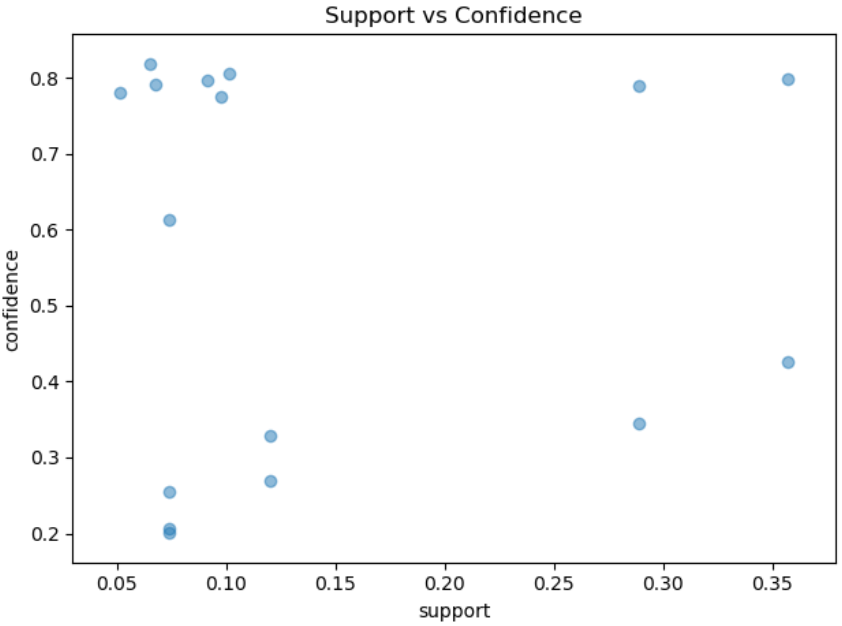
\includegraphics[scale=0.45]{images/support_vs_confidence.png}\\
\caption{Support vs Confidence}
\label{Fig_1} 
\end{figure}

\begin{figure}[H]
\centering
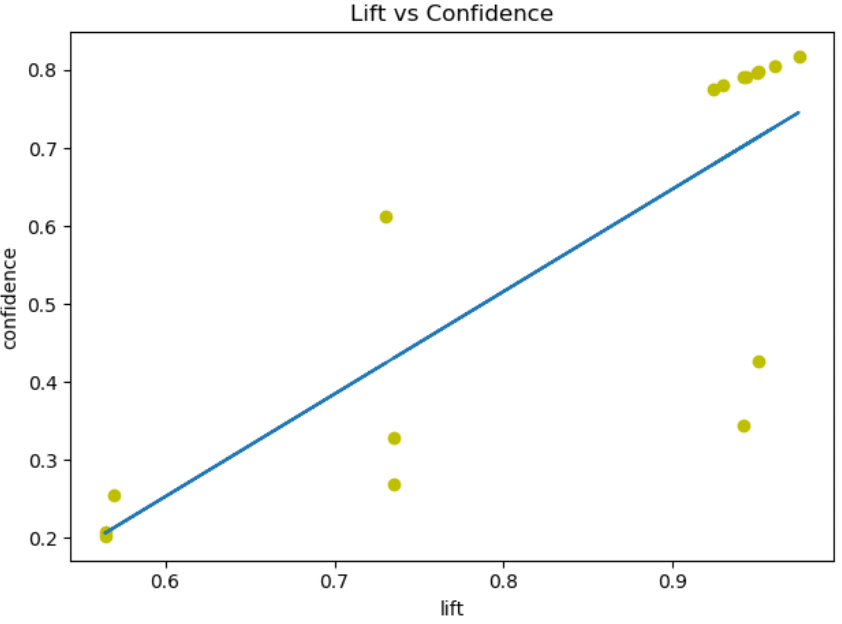
\includegraphics[scale=0.45]{images/lift_vs_confidence.png}
\caption{Lift vs Confidence}
\label{Fig_2} 
\end{figure}


\section{Conclusions \& Discussion}

Our project sheds light on how to build more successful recommendation systems for clothes. Our work shows that human could capture linguistic cues from customer reviews to predict why customers bought the product. Theoretically, our work contributes to the understanding of customers' personal disclosure during purchasing. Moreover, we proposed several computational models to allow this exploration in large scales. Furthermore, we also analyze the inner relationship between different types of items based on the association rules to make a comprehensive recommendation systems.

The challenges we faced includes:
\begin{itemize}
    \item Dirty data with lots of null, meaningless words, meaningless characters in customer's reviews.
    \item Dealing with unbalanced data that would cause bias on the items with high numbers.
    \item Brainstorming about inner relationship of our data set and pick up the idea to make recommendation system for online renting platform.
\end{itemize}
We learnt:
\begin{itemize}
    \item The on-hand data preprocessing skills to deal with the dirty data.
    \item Practical methods for mining values from large scale datasets like techniques discussed above.
  \end{itemize}
We loves every parts of our project, especially when we learned that we would not have a final exam thanks to this project. Specifically, we enjoy reading creative comments and jokes in customer reviews.

Both members participates in the brainstorming. Jiajun Bao wrote the introduction, section 3.1 and 3.2. Qinyun wrote section 2 and section 3.3. Both members participates in writing the rest parts. 
Jiajun Bao worked on the hattn and ALBERT methods, and human annotation. Qinyun worked on the data filtering, SVM methods, and associated rule learning.
\bibliographystyle{acm}
\bibliography{references}

\end{document}


